\documentclass[a4paper, 11pt]{article}

\usepackage[utf8]{inputenc}
\usepackage[T1, T2A]{fontenc}
\usepackage[english, russian]{babel}

\usepackage[top=2cm, bottom=2cm, left=2cm, right=2cm]{geometry}
\usepackage{graphicx}

\usepackage{pgfplots}
\pgfplotsset{compat=1.13}
\pgfplotsset{grid = major, grid style = {dashed}}

%Change label separator
\usepackage{caption}
\captionsetup[table]{labelformat=simple, labelsep = endash}
\captionsetup[figure]{labelformat=simple, labelsep = endash}

\usepackage{subcaption}

\usepackage{amsmath}

\usepackage{../titlepage/TAYTitle}
\author{Овчаров Алексей}
\title{Экспериментальное построение областей устойчивости линейной системы на плоскости двух параметров}
\labnumber{8}
\variant{3}

\begin{document}
\maketitle

\paragraph{Цель работы.}Ознакомление с экспериментальными методами построения областей устойчивости линейных динамических систем и изучение влияния на устойчивость системы ее параметров.

\paragraph{Исходные данные.} Необходимо исследовать систему при $g = 0$, $y(0) = 1$ и $T_1 = 1$. Сама система представлена на следующем рисунке.
\begin{figure}[h!]
    \centering
    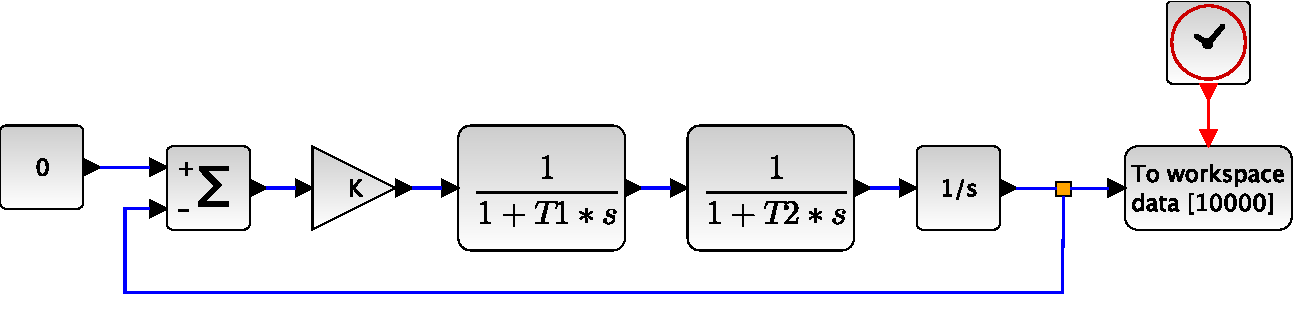
\includegraphics[width = 0.8\textwidth]{images/model.pdf}
    \caption{Исследуемая система.}
\end{figure}
\section*{Устойчивость системы}
На риунке 2 показаны преходные характеристики системы при различный $k$ и $T_2 = 0.1$. Соответственно на рисунке 1 (а) при $k = 1$, (b) при $k = 0$, (c) при $k = 11$, (d) при $k = 25$.
\begin{figure}[h!]
    \begin{subfigure}[b]{0.5\textwidth} 
        \centering
        \begin{tikzpicture}
            \begin{axis}[
                width = 0.9\textwidth,
                extra y ticks = {0},
                extra tick style={grid=major},
                xlabel = {$t, c$},
                ylabel = {$y$},
            ]
                \addplot[color=black, mark=none, style=thick] table {data/dataStabel.dat};
            \end{axis}
        \end{tikzpicture}
        \caption{Устойчивая система.}
    \end{subfigure}
    \begin{subfigure}[b]{0.5\textwidth} 
        \centering
        \begin{tikzpicture}
            \begin{axis}[
                width = 0.9\textwidth,
                xlabel = {$t, c$},
                ylabel = {$y$},
            ]
                \addplot[color=black, style=thick] coordinates {(0, 1) (30, 1)};
            \end{axis}
        \end{tikzpicture}
       \caption{Граница устойчивости нейтрального типа.}
    \end{subfigure}

    \vspace{0.5cm} 

    \begin{subfigure}[b]{0.5\textwidth} 
        \centering
        \begin{tikzpicture}
            \begin{axis}[
                width = 0.9\textwidth,
                extra y ticks = {0},
                extra tick style={grid=major},
                xlabel = {$t, c$},
                ylabel = {$y$},
            ]
                \addplot[color=black, mark=none, style=thick] table {data/dataVibrating.dat};
            \end{axis}
        \end{tikzpicture}
        \caption{Граница устойчивости колебательного типа.}
    \end{subfigure}
    \begin{subfigure}[b]{0.5\textwidth} 
        \centering
        \begin{tikzpicture}
            \begin{axis}[
                width = 0.9\textwidth,
                extra y ticks = {0},
                extra tick style={grid=major},
                xlabel = {$t, c$},
                ylabel = {$y$},
            ]
                \addplot[color=black, mark=none, style=thick] table {data/dataNoStable.dat};
            \end{axis}
        \end{tikzpicture}
       \caption{Неустойчивая система.}
    \end{subfigure}
    \caption{Устойчивость системы.}
\end{figure}

\section*{Анализ устойчивости системы}
Предаточная функция исходной сисемы выглядит следющим образом:
\begin{equation}
    W(s) = \frac{K}{T_1 T_2 s^3 + (T_1 + T_2)s^2 + s + K}
\end{equation}
Для анализа устойчивости системы составим матрицу Гурвица.

\begin{equation}
    H_3 = \begin{bmatrix}
        T_1 + T_2 &  K & 0 \\
        T_1 T_2 & 1 & 0 \\
        0 & T_1 + T_2 & 1
    \end{bmatrix}
\end{equation}

Из этой матрицы можем, исользуя условие Гурвица, получить уравнение для системы на границы устойчивости колебательного типа.
\begin{equation}
    \begin{cases}
        T_1 + T_2 - K T_1 T_2 = 0 \\
        T_1 + T_2 > 0 \\
        K > 0
    \end{cases}
\end{equation}

А также можно получить условие для системы на границе устойчивости нейтрального типа.
\begin{equation}
    K = 0 \\
\end{equation}

Получив все необходимые уравнения мы можем построить график зависимости $K(T_2)$, $T_2 \in [0.1, 5]$. Как видно из уравнения (2) - эта зависимость является гиперболой, в случае же уравнения (3) - просто прямой $K = 0$, $T_2 \in (-\infty, +\infty)$. График данной зависимости представлен ниже на рисунке 3.
\begin{figure}[h!]
    \centering
    \begin{tikzpicture}
        \begin{axis}[
            width = 0.8\textwidth,
            height = 7cm,
            xlabel = {$T_2$},
            ylabel = {$K$},
        ]
            \addplot[color=black, mark=none, style=thick] table {data/dataTreshold.dat};
            \addplot[color=black, mark=none, style=thick] coordinates {(0.1, 0) (5, 0)};
        \end{axis}
    \end{tikzpicture}
    \caption{График границы устойчивости $K(T_2)$.}
\end{figure}
\section*{Выводы}
В данной работе мы экспериметнально и аналитически оценили устойчивость систему варьируя ее параметры $K$ и $T_2$, зафиксировав при этом $T_1$. Аналитическую оценку позволил получить критерий Гурциа. Соотвественно по составленной матрице (2) мы смогли получить и составить условия границы устойчивоси (3) и (4), после чего убедились в правильности полученных экспериментальных значений.
\end{document}
